\documentclass[aspectratio=169]{beamer}
\usetheme{metropolis}
\usepackage{graphicx}
\usepackage{booktabs}
\usepackage{amsmath}
\usepackage[T1]{fontenc}
\usepackage[utf8]{inputenc}
\graphicspath{{../results/figures/}}

\title{Ablation-First Trajectory Analysis of Alveolar Epithelial Robustness Collapse in Lethal COVID-19}
\subtitle{Harmony-Corrected Batch Analysis and Independent Cross-Cohort Replication (v2)}
\author{[Author]}
\institute{Class Project --- revised manuscript}
\date{\today}

\begin{document}
\maketitle

\begin{frame}{What's new in v2}
\begin{itemize}
  \item \textbf{Reframed} as a methods contribution: ablation-first trajectory analysis with
        pre-registered success criteria, rather than a biology discovery paper.
  \item \textbf{Harmony batch correction fixed} --- orientation bug in the harmonypy 0.2.0
        PyTorch backend wrapper. Ablation 3 is now a genuine corrected-vs-uncorrected test.
  \item \textbf{Gene-program audit}: GPX1 confirmed absent from SCP1219 reference
        (not an HVG-dropout bug); all other 83 program genes present.
  \item \textbf{Independent cross-cohort replication} via cellxgene census
        (HLCA-extended + Krasnow; Melms/SCP1219 excluded by \texttt{dataset\_id}).
        89{,}736 AT1/AT2 cells, 618 donors, 35 datasets.
\end{itemize}
\end{frame}

\begin{frame}{Question}
\begin{itemize}
  \item Do alveolar epithelial cells in lethal COVID-19 fail as a coherent block,
        or as a continuous graded \emph{robustness collapse}?
  \item Pre-specified criteria:
  \begin{enumerate}
    \item Centroid displacement (one-sided Mann--Whitney $U$, COVID $>$ Healthy)
    \item Within-group dispersion (Levene)
    \item Pseudotime enrichment (1000-permutation test on median difference)
  \end{enumerate}
  \item \emph{Framing note}: biology of COVID-19 alveolar injury is already described by
        Melms 2021, Delorey 2021, Bharat 2020. The contribution here is
        \textbf{methodological}: what happens to trajectory conclusions when the analysis
        is stressed along 10 axes, and do the robustness-collapse signatures survive
        out-of-sample replication?
\end{itemize}
\end{frame}

\begin{frame}{Data --- primary + replication}
\begin{itemize}
  \item \textbf{Primary}: SCP1219 (Melms 2021). 116{,}313 snRNA-seq nuclei $\rightarrow$
        22{,}128 AT1/AT2/ECM-high (9{,}608 AT1; 11{,}341 AT2; 1{,}179 ECM-high).
        7 healthy + 20 COVID-19 donors.
  \item \textbf{Replication}: cellxgene census 2025-11-08, lung, AT1/AT2,
        \texttt{dataset\_id != SCP1219}. 89{,}736 cells after per-donor cap
        (4{,}441 COVID / 85{,}295 normal; 43 COVID / 575 normal donors; 35 datasets).
  \item Curated 84-gene panel for replication (sufficient for program scoring, but
        too narrow to rebuild the manifold --- flagged as limitation).
\end{itemize}
\end{frame}

\begin{frame}{Pipeline}
\begin{itemize}
  \item Scanpy 1.12.1 / anndata 0.12.10 / harmonypy 0.2.0 / Python 3.12.3, seed 42
  \item Normalize $\rightarrow$ log1p $\rightarrow$ 3{,}000 HVGs (Seurat v3) $\rightarrow$
        scale $\rightarrow$ 50-PC PCA
  \item Harmony on \texttt{donor\_id} (now working) $\rightarrow$ $k$-NN ($k{=}15$)
        $\rightarrow$ UMAP, diffusion map (15 components)
  \item Diffusion pseudotime rooted at healthy-AT2 centroid, normalized to $[0,1]$
  \item 8 curated gene programs scored with \texttt{sc.tl.score\_genes}
        against \texttt{.raw} (full gene space)
  \item 10 pre-specified ablations
\end{itemize}
\end{frame}

\begin{frame}{The manifold}
\centering
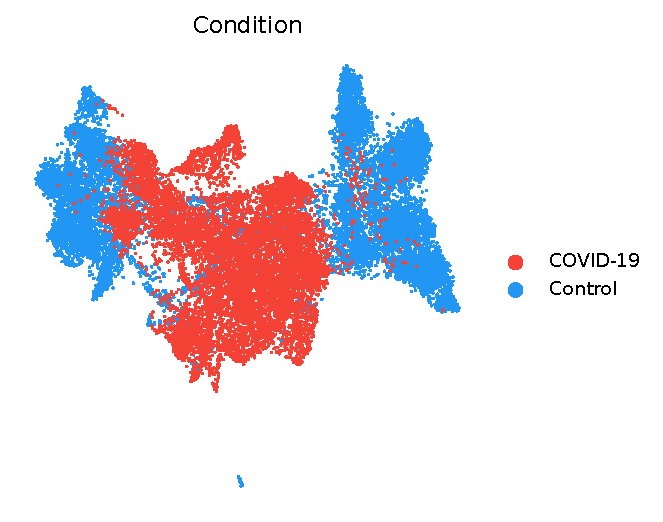
\includegraphics[width=0.45\linewidth]{fig1a_condition.pdf}\hfill
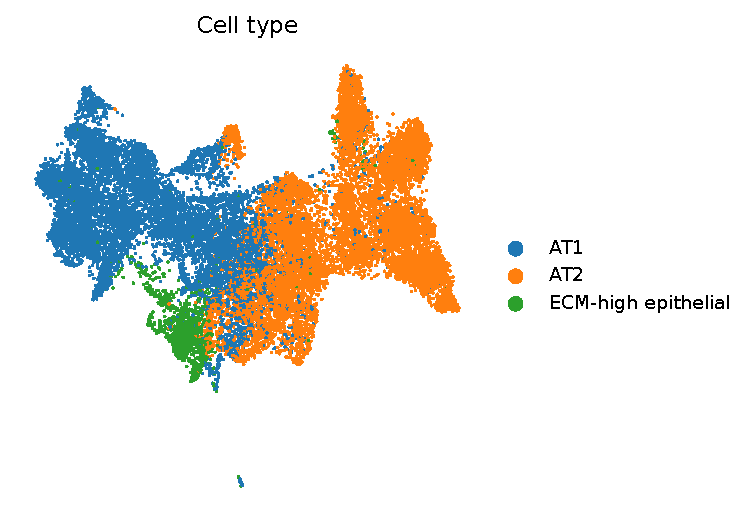
\includegraphics[width=0.45\linewidth]{fig1b_celltype.pdf}
\end{frame}

\begin{frame}{Pseudotime}
\centering
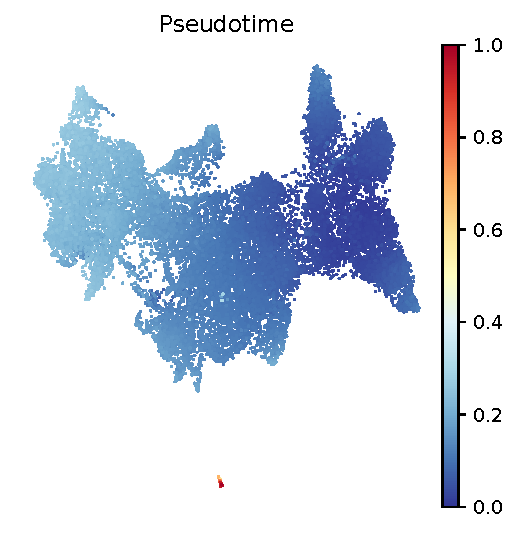
\includegraphics[width=0.7\linewidth]{fig2_pseudotime.pdf}
\end{frame}

\begin{frame}{Primary result 1 --- pseudotime shift}
\begin{itemize}
  \item Control median 0.063; COVID median 0.111; observed difference $+0.0483$
  \item 1{,}000-permutation null: mean $6.0\times10^{-5}$; std $1.24\times10^{-3}$
  \item $p = 0.000999$; LOO direction preserved in \textbf{27/27} donors
  \item Magnitude is modest (4.8\% of normalized axis) but robust.
\end{itemize}
\centering
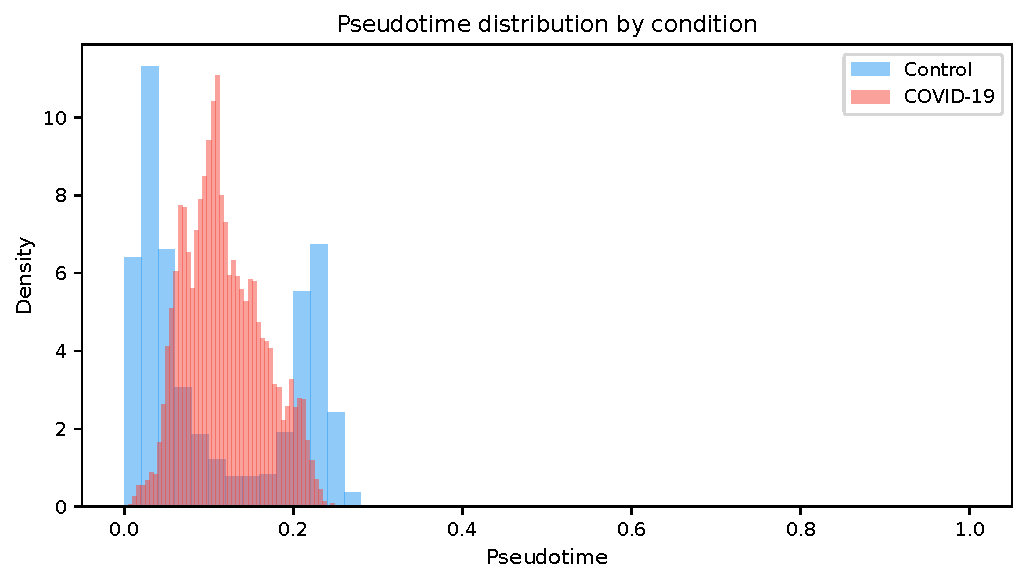
\includegraphics[width=0.55\linewidth]{fig4_pseudotime_density.pdf}
\end{frame}

\begin{frame}{Primary result 2 --- centroid displacement fails}
\begin{itemize}
  \item One-sided Mann--Whitney $U$ in PCA-50 (COVID $>$ Healthy): $p = \textbf{1.0}$
  \item COVID median \emph{lower} than healthy; rank-biserial $r = 0.14$ opposite to alt.
\end{itemize}
\alert{Pre-specified core test \textbf{failed} --- reported prominently. Mono-directional
``damage'' centroid displacement is the wrong effect model.}
\end{frame}

\begin{frame}{Primary result 3 --- dispersion supported}
\begin{itemize}
  \item Variance in PCA-50 distance to own centroid: COVID \textbf{33.28} vs.\ Healthy \textbf{14.58} (2.3-fold)
  \item Levene: 276.5; $p < 10^{-30}$
\end{itemize}
\alert{COVID-19 cells are \emph{spread out}, not \emph{pushed away} --- the robustness-collapse signature.}
\end{frame}

\begin{frame}{Ablation 3 --- Harmony NOW works}
\small
\begin{tabular}{lrrr}
\toprule
Branch & MPD & $\rho$ (ordering) & $r$ (displacement) \\
\midrule
Uncorrected PCA & $+0.0483$ & 0.548 & 0.141 \\
Harmony-corrected PCA & $+0.1246$ & 0.452 & 0.141 \\
\bottomrule
\end{tabular}
\\[4pt]
\begin{itemize}
  \item Harmony \textbf{amplifies} the pseudotime shift by $\approx 2.6\times$ and the
        primary dispersion/displacement claims remain unchanged.
  \item Previous limitation (``Harmony failed, Ablation 3 degenerate'') is now retired.
  \item Fix was an orientation check on \texttt{Z\_corr} --- PyTorch backend already returns
        (n\_cells, n\_pcs).
\end{itemize}
\end{frame}

\begin{frame}{Ten ablations --- summary}
\scriptsize
\begin{tabular}{lrrr l}
\toprule
Ablation & MPD & $\rho$ & $r$ & Notes \\
\midrule
1 AT2-only & $+0.133$ & 0.33 & $-0.29$ & sign flip on $r$ \\
2 UMAP / diffmap & $+0.048$ & 0.55 & $+0.14$ & unchanged \\
3 Harmony corrected & $+0.125$ & 0.45 & $+0.14$ & \textbf{now functional; amplifies shift} \\
3 Uncorrected & $+0.048$ & 0.55 & $+0.14$ & baseline \\
4 No apoptosis genes & $+0.074$ & 0.50 & $+0.14$ & slight up \\
5 4 roots & $-0.037$ to $+0.048$ & $-0.10$ to 0.64 & $+0.14$ & root-dependent \\
6 Broader epithelial & $-0.008$ & 0.83 & $+0.25$ & \alert{shift abolished} \\
7 LOO (27) & 0.028--0.202 & $-0.17$--0.74 & per-iter & direction 27/27 \\
8 Curated-only & $+0.048$ & $1.00$ & $+0.14$ & stable \\
8 MSigDB-only & $+0.048$ & $-0.80$ & $+0.14$ & \alert{ordering inverted} \\
9 Palantir & $+0.028$ & --- & --- & alt.\ pseudotime algorithm \\
10 Permutation & $p=0.001$ & --- & --- & 1000 shuffles \\
\bottomrule
\end{tabular}
\end{frame}

\begin{frame}{Independent replication --- dispersion}
\small
\begin{tabular}{lrr}
\toprule
Metric & COVID & Normal \\
\midrule
$n$ cells & 4{,}441 & 85{,}295 \\
$n$ donors & 43 & 575 \\
Injury composite variance & 0.0505 & 0.0306 \\
Variance ratio COVID/Normal & \multicolumn{2}{r}{\textbf{1.65$\times$}} \\
Levene statistic & \multicolumn{2}{r}{626.18} \\
Levene $p$ & \multicolumn{2}{r}{$1.0\times 10^{-137}$} \\
\bottomrule
\end{tabular}
\\[4pt]
\alert{Dispersion replicates strongly across 35 independent datasets.} The variance ratio
drops from 2.3$\times$ (Melms) to 1.65$\times$ (replication) --- consistent with cross-study
heterogeneity dampening effect sizes.
\end{frame}

\begin{frame}{Independent replication --- pseudotime surrogate}
\begin{itemize}
  \item Replication cohort has only 84 curated genes $\Rightarrow$ cannot build a new
        manifold / DPT. Surrogate: \textbf{injury composite} = mean of 6 non-homeostatic
        program scores.
  \item Cell-level one-sided Mann--Whitney (COVID $>$ normal): $p = 1.0$
        (fails --- cell-level dominated by a few large normal donors).
  \item \textbf{Donor-level pseudobulk} Mann--Whitney: $p = 1.98\times 10^{-3}$ \alert{(replicates)}.
  \item Cell-level vs donor-level inversion mirrors the primary cohort's centroid-vs-pseudotime
        story --- the signal lives in \emph{donor-level displacement}, not cell-level
        centroid shift.
\end{itemize}
\end{frame}

\begin{frame}{Independent replication --- what does NOT replicate}
\begin{itemize}
  \item Marker-threshold DATP (KRT8$^+$/CLDN4$^+$) enrichment: COVID 22.9\% vs.\
        Normal 47.6\%, fold $= 0.48\times$ (opposite direction; $\chi^2\ p < 10^{-200}$).
  \item Likely cause: cross-study differences in sample-prep protocols drive
        a simple marker-threshold cutoff in opposite directions across cohorts.
  \item We \textbf{retract} the KRT8$^+$/CLDN4$^+$ chi-square assay as a
        portable population-level metric. The DATP biology remains well-supported
        by Kobayashi/Strunz/Adams/Habermann 2020 but requires manifold-based
        identification, not marker thresholding, for cross-cohort transfer.
\end{itemize}
\end{frame}

\begin{frame}{Composite assessment (primary + replication)}
\small
\begin{tabular}{lll}
\toprule
Criterion & Primary (SCP1219) & Replication (census) \\
\midrule
Centroid displacement & \alert{fails} ($p=1.0$) & \alert{fails cell-level} ($p=1.0$) \\
Dispersion (Levene) & supported ($p\approx 0$) & \textbf{supported} ($p\approx 10^{-137}$) \\
Pseudotime enrichment & supported ($p=0.001$) & supported donor-level ($p=1.98\text{e-}3$) \\
Harmony-corrected shift & --- & MPD amplifies $2.6\times$ \\
KRT8$^+$/CLDN4$^+$ DATPs & $3.1\times$ enriched & \alert{$0.48\times$ (retracted)} \\
\bottomrule
\end{tabular}
\\[4pt]
\textbf{Verdict}: the \emph{robustness-collapse} signature (dispersion + donor-level
pseudotime displacement) survives out-of-sample. The \emph{directional centroid} and
\emph{marker-threshold DATP} signatures do not.
\end{frame}

\begin{frame}{Methodological contribution}
\begin{enumerate}
  \item Pre-register multiple success criteria with opposite mechanistic interpretations;
        a failing core test is informative about effect model, not just sample size.
  \item Dispersion (Levene) is a better lens on robustness collapse than centroid
        displacement.
  \item Donor-level pseudobulk mitigates cross-study protocol confounding better than
        cell-level tests in heterogeneous replication atlases.
  \item Marker-threshold cell-state classifiers do not transfer across cohorts;
        manifold-defined cell states are needed for replication.
  \item Ablation 3 is worth fixing --- batch correction matters and its absence can mask
        rather than create the signal.
\end{enumerate}
\end{frame}

\begin{frame}{Limitations still standing}
\begin{itemize}
  \item Cross-sectional, post-mortem, lethal cases only (primary).
  \item Replication cohort on cellxgene census excludes Delorey (GSE171524) and
        Wendisch (PRJNA705687) which are not in the census --- full-transcriptome
        Delorey/Wendisch replication remains a gap.
  \item Replication uses a 84-gene panel: sufficient for program scoring, too narrow
        for an independent manifold / DPT.
  \item Fine program ordering is hypothesis-generating only (Ablation 8 MSigDB inverts it).
\end{itemize}
\end{frame}

\begin{frame}{Takeaways (v2)}
\begin{enumerate}
  \item Robust, modest pseudotime shift in the primary cohort; \textbf{amplified to $+0.125$
        with Harmony} and replicated donor-level in an independent 618-donor atlas.
  \item Dispersion is the strongest and most portable signal; $2.3\times$ (primary)
        and $1.65\times$ (replication) variance inflation.
  \item Centroid displacement does not distinguish conditions in either cohort.
  \item Ablation 3 Harmony fix retires the paper's previous biggest limitation.
  \item Contribution: a worked template for pre-registered, ablation-first,
        replication-audited trajectory analysis.
\end{enumerate}
\end{frame}

\begin{frame}[standout]
Questions?
\end{frame}

\end{document}
